\documentclass[pdf]{beamer}
\usetheme{CambridgeUS}
\definecolor{WiLabRed}{RGB}{197,18,48}
                               \setbeamercolor{frametitle}{fg=white,bg=WiLabRed}
\setbeamercolor{progress bar}{fg=WiLabRed!90}
\setbeamercolor{palette tertiary}{fg=white,bg=WiLabRed}
\setbeamercolor{title separator}{fg=WiLabRed!90}
\setbeamercolor{progress bar in section page}{fg=WiLabRed!90}
\setbeamercolor{background canvas}{bg=white}
\setbeamercolor{alerted text}{fg=WiLabRed!90}
\setbeamertemplate{headline}


\setbeamertemplate{footline}
{
  \leavevmode%
  \hbox{%
  \begin{beamercolorbox}[wd=.3\paperwidth,ht=2.25ex,dp=1ex,center]{author in head/foot}%
    \usebeamerfont{author in head/foot}Kyle W. McClintick
  \end{beamercolorbox}%
  \begin{beamercolorbox}[wd=.6\paperwidth,ht=2.25ex,dp=1ex,center]{title in head/foot}%
    \usebeamerfont{title in head/foot}Email: \Letter kwmcclintick@wpi.edu
  \end{beamercolorbox}%
  \begin{beamercolorbox}[wd=.1\paperwidth,ht=2.25ex,dp=1ex,center]{date in head/foot}%
    \insertframenumber{} / \inserttotalframenumber\hspace*{1ex}
  \end{beamercolorbox}}%
  \vskip0pt%
}

\usepackage{xcolor}
\usepackage{appendixnumberbeamer}
\usepackage{booktabs}
\usepackage{hyperref}
\usepackage{wrapfig}
\usepackage[scale=2]{ccicons}
\usepackage{pgfplots}
\usepgfplotslibrary{dateplot}
\usepackage{xspace}
\newcommand{\themename}{\textbf{\textsc{metropolis}}\xspace}
\graphicspath{{./Images/}{./Misc/}}
\usepackage{marvosym}
\usepackage{subfig}
\usepackage{graphicx}
\usepackage{verbatim}
\usepackage{caption}


\title{An Analysis of Recurrent Neural Networks forBotnet Detection Behavior}
\date{April 29th, 2020}
\author{\textbf{Kyle McClintick} \small{\\ Dept. of Electrical \& Computer Engineering, Worcester Polytechnic Institute, Worcester, MA 01609 USA}}
\vspace{-20cm}
\institute{ \hfill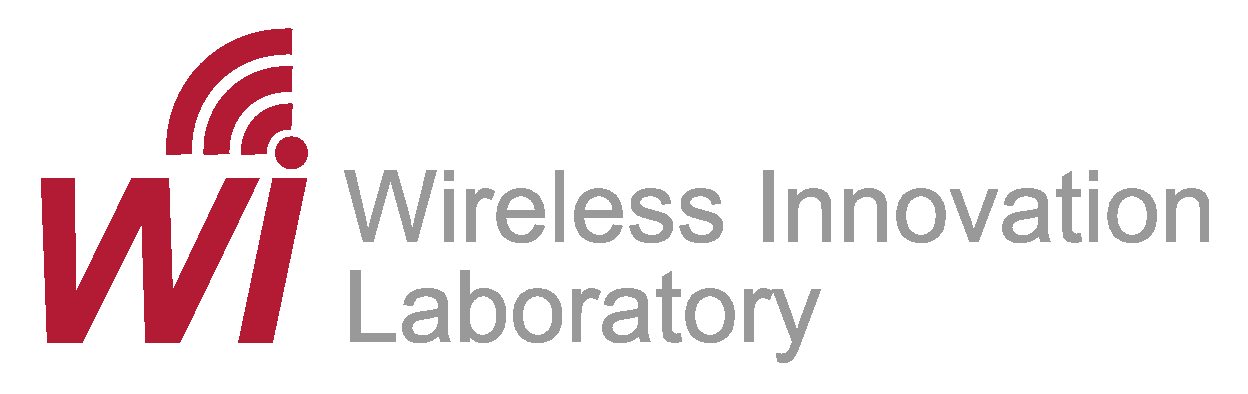
\includegraphics[height=1.5cm]{wilab_logo-A70916.eps}\hspace*{1.7cm}
\includegraphics[height=1.5cm]{WPI_Inst_Prim_FulClr.eps}}

\usepackage{csquotes}
\usepackage[style=verbose-ibid,backend=bibtex]{biblatex}
\bibliography{myreferences.bib}


\begin{document}

\captionsetup[subfigure]{labelformat=empty}

\maketitle






%%%%%%%%%%%%%%%%%%%%%%%%%%%%%%%%%%%%%%%%%%%%%%%%%%%%%%%%%%%%%%%%%%%%%%
\begin{frame}[fragile]{Brief History}
\begin{minipage}[0.2\textheight]{\textwidth}
\begin{columns}[T]
\begin{column}{0.5\textwidth}
\begin{itemize}
\item 2014: DDoS attacks on competing Minecraft servers under the pseudonym “lelddos”
\item 2016: French hosting company OVH suffered a DDoS attack with a total capacity of up to 1.5 terabits per second
\item Co-developer published the source code under the name “Anna-Senpai”. Many hackers copied and developed the code.
\item Largest DDoS attack ever launched, targeting the DNS provider “Dyn”. Amazon, Netflix and Spotify, were unavailable for a long time
\end{itemize}
\end{column}
\begin{column}{0.5\textwidth}
\vspace{2cm}
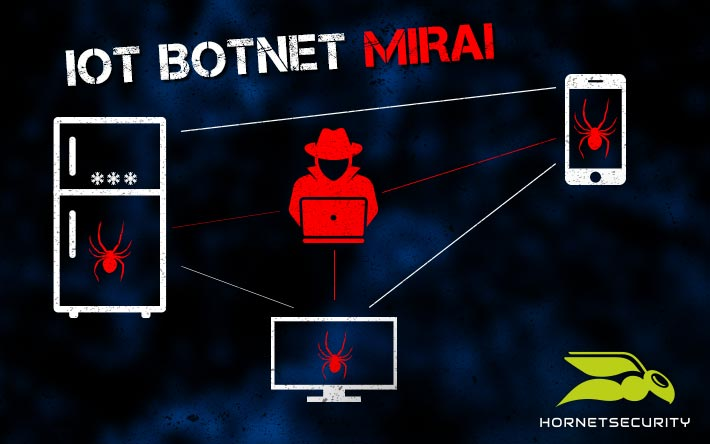
\includegraphics[width=5cm]{Images/mirai.jpg}
\end{column}
\end{columns}
\end{minipage}
\end{frame}



%%%%%%%%%%%%%%%%%%%%%%%%%%%%%%%%%%%%%%%%%%%%%%%%%%%%%%%%%%%%%%%%%%%%%%
\begin{frame}[fragile]{Brief History}
\begin{minipage}[0.2\textheight]{\textwidth}
\begin{columns}[T]
\begin{column}{0.5\textwidth}
\begin{itemize}
\item FBI involved, three Alaskans pleaded guilty and avoided jail time by manditory employment with the FBI to counter botnet of things attacks
\item 2019: bot net of things attacks have returned with 11 new exploits (27 total now) spreads primarily through presentation systems, smart TVs, routers and IP cameras
\end{itemize}
\end{column}
\begin{column}{0.5\textwidth}
\vspace{1cm}
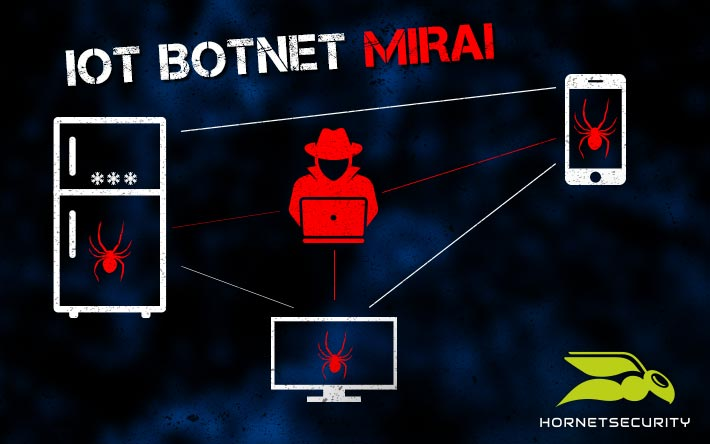
\includegraphics[width=5cm]{Images/mirai.jpg}
\end{column}
\end{columns}
\end{minipage}
\end{frame}


%%%%%%%%%%%%%%%%%%%%%%%%%%%%%%%%%%%%%%%%%%%%%%%%%%%%%%%%%%%%%%%%%%%%%%
\begin{frame}[fragile]{Personal Interest}
\begin{minipage}[0.2\textheight]{\textwidth}
\begin{columns}[T]
\begin{column}{0.75\textwidth}
DARPA’s Open Programmable Secure 5G (OPS-5G) program will create open source software and systems enabling secure 5G and follow-on mobile networks. OPS-5G creates capabilities to address feature velocity in open source software, a trillion-node Botnet of Things (BoT), network slicing on suspect gear and adaptive adversaries operating at scale. The long-term objective is a US-friendly ecosystem.
\end{column}
\begin{column}{0.25\textwidth}
\vspace{1cm}

\includegraphics[width=2.5cm]{Images/darpa.jpg}
\end{column}
\end{columns}
\end{minipage}
\end{frame}


%%%%%%%%%%%%%%%%%%%%%%%%%%%%%%%%%%%%%%%%%%%%%%%%%%%%%%%%%%%%%%%%%%%%%%
\begin{frame}[fragile]{Agenda}
\begin{minipage}[0.2\textheight]{\textwidth}
\begin{columns}[T]
\begin{column}{0.5\textwidth}
\begin{itemize}
\item Abstract
\item Key Contributions
\item State of the Art
\item Novel Method
\item Results
\item Conclusion
\end{itemize}
\end{column}
\begin{column}{0.5\textwidth}

\includegraphics[width=5cm]{Images/agenda.png}
\end{column}
\end{columns}
\end{minipage}
\end{frame}




%%%%%%%%%%%%%%%%%%%%%%%%%%%%%%%%%%%%%%%%%%%%%%%%%%%%%%%%%%%%%%%%%%%%%%
\begin{frame}[fragile]{Abstract}
\begin{figure}

\includegraphics[width=0.3\linewidth,keepaspectratio]{Images/botnet.png}
\caption{A Botnet can be conceived as a group of compromised computers which can be controlled remotely to execute coordinated  attacks  or  commit  fraudulent  acts.  The  fact  that Botnets     continuously   evolve   means   that   traditional detection  approaches  are  always  one  step  behind. }
\end{figure}
\end{frame}

%%%%%%%%%%%%%%%%%%%%%%%%%%%%%%%%%%%%%%%%%%%%%%%%%%%%%%%%%%%%%%%%%%%%%%
\begin{frame}[fragile]{Abstract}
\begin{figure}
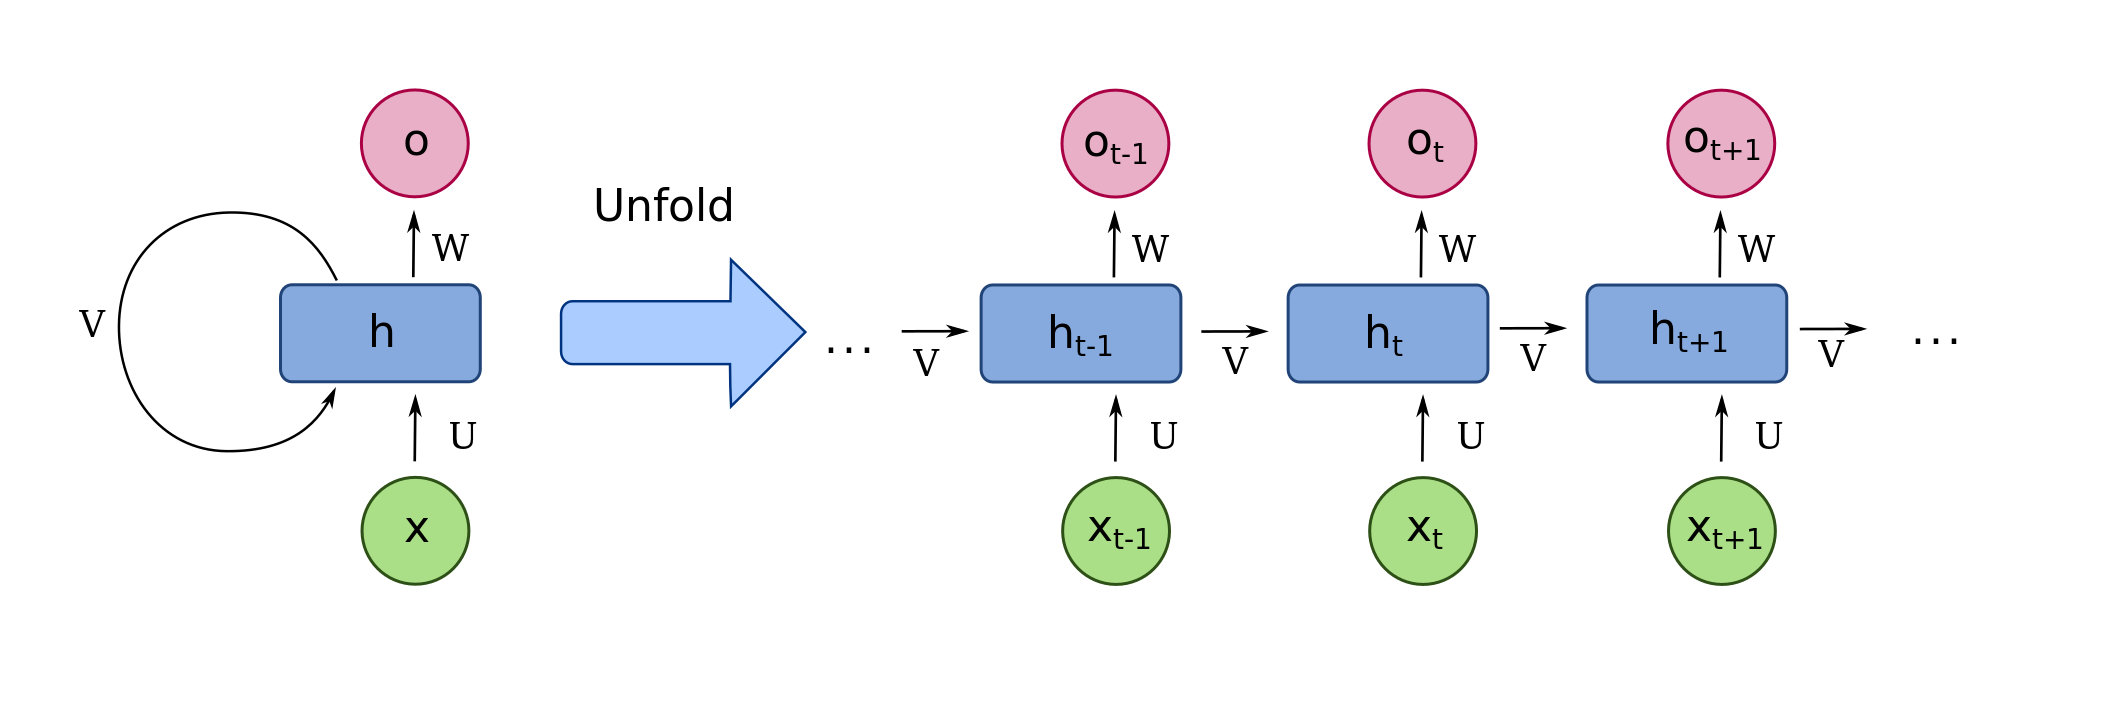
\includegraphics[width=0.9\linewidth,keepaspectratio]{Images/rnn.png}
\caption{Temporal analysis of  network behavior, specifically duration and load of network traffic from different nodes, can be used to infer if a node is part of a botnet attack. Using Recurrent Neural Networks, preliminary are good.  However,  experiments  exposed that experimental data is too similar to classify accurately.}
\end{figure}
\end{frame}





%%%%%%%%%%%%%%%%%%%%%%%%%%%%%%%%%%%%%%%%%%%%%%%%%%%%%%%%%%%%%%%%%%%%%%
\begin{frame}[fragile]{Key Contributions}
\begin{minipage}[0.2\textheight]{\textwidth}
\begin{columns}[T]
\begin{column}{0.5\textwidth}
\begin{itemize}
\item A better model: state of the Art is the Strastosphere Intrusion Prevention System (IPS) project, a first order Markov Model, which struggles to sample large state spaces, and only makes predictions using the pervious state
\item All bots must receive instructions from the bot master at some point, can this sparse, long-sequence behavior be recognized?
\end{itemize}
\end{column}
\begin{column}{0.5\textwidth}

\includegraphics[width=5cm]{Images/contribute.png}
\end{column}
\end{columns}
\end{minipage}
\end{frame}







%%%%%%%%%%%%%%%%%%%%%%%%%%%%%%%%%%%%%%%%%%%%%%%%%%%%%%%%%%%%%%%%%%%%%%
\begin{frame}[fragile]{State of The Art}
\begin{minipage}[0.2\textheight]{\textwidth}
\begin{columns}[T]
\begin{column}{0.5\textwidth}
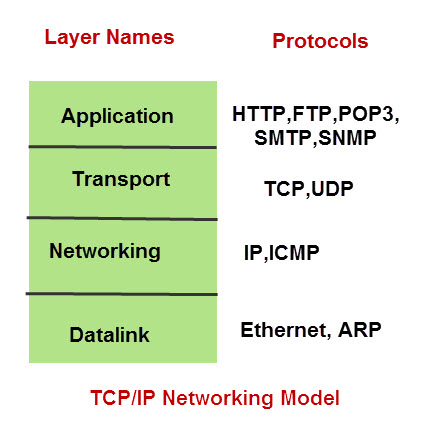
\includegraphics[width=6cm]{Images/suite.jpg}
\end{column}
\begin{column}{0.5\textwidth}
\vspace{2cm}
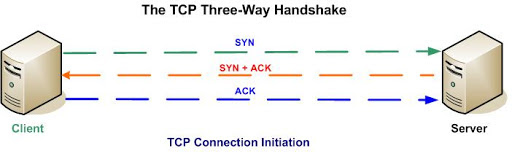
\includegraphics[width=6cm]{Images/tcp.jpg}
\end{column}
\end{columns}
\end{minipage}
\end{frame}


%%%%%%%%%%%%%%%%%%%%%%%%%%%%%%%%%%%%%%%%%%%%%%%%%%%%%%%%%%%%%%%%%%%%%%
\begin{frame}[fragile]{State of The Art}
\begin{figure}
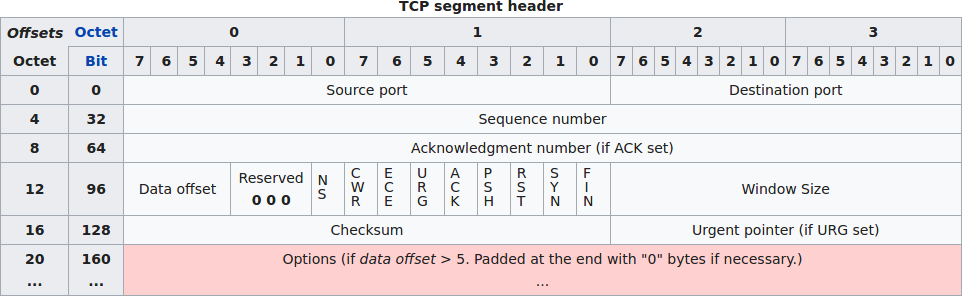
\includegraphics[width=1\linewidth,keepaspectratio]{Images/tcp_head.png}
\end{figure}
\end{frame}


%%%%%%%%%%%%%%%%%%%%%%%%%%%%%%%%%%%%%%%%%%%%%%%%%%%%%%%%%%%%%%%%%%%%%%
\begin{frame}[fragile]{State of The Art}
\begin{minipage}[0.2\textheight]{\textwidth}
\begin{columns}[T]
\begin{column}{0.5\textwidth}
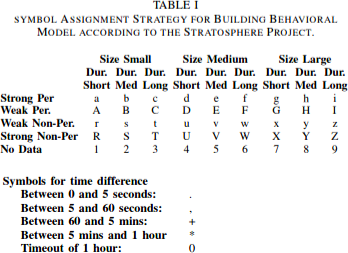
\includegraphics[width=6cm]{Images/behavior.png}
\end{column}
\begin{column}{0.5\textwidth}
\vspace{2cm}
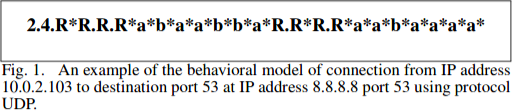
\includegraphics[width=6cm]{Images/example.png}
\end{column}
\end{columns}
\end{minipage}
\end{frame}


%%%%%%%%%%%%%%%%%%%%%%%%%%%%%%%%%%%%%%%%%%%%%%%%%%%%%%%%%%%%%%%%%%%%%%
\begin{frame}[fragile]{Novel Method: Data Representation}
\begin{minipage}[0.2\textheight]{\textwidth}
\begin{columns}[T]
\begin{column}{0.5\textwidth}
\begin{itemize}
\item Data: 50 different possible states, each state is grouped into a length $n$ sequence $X_{n,t} \in \{ 0, 1 \}^{50}$. A connection can have any number of sequences.
\item Labels: Binary classification, normal or botnet. $Y_t \in \{ 0,1 \}$
\item Collection: TCP/IP connections between computers at Czech technical university in Prague.
\end{itemize}
\end{column}
\begin{column}{0.5\textwidth}
\vspace{1cm}
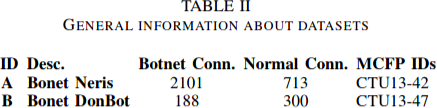
\includegraphics[width=6cm]{Images/table2.png}
\end{column}
\end{columns}
\end{minipage}
\end{frame}


%%%%%%%%%%%%%%%%%%%%%%%%%%%%%%%%%%%%%%%%%%%%%%%%%%%%%%%%%%%%%%%%%%%%%%
\begin{frame}[fragile]{Novel Method: Challenges}
\begin{minipage}[0.2\textheight]{\textwidth}
\begin{columns}[T]
\begin{column}{0.5\textwidth}
\begin{itemize}
\item Architecture: while LSTM has the capability to classify outcomes using states from millions of time steps ago, there is no generative approach to implement this
\item Class imbalance: many more normal states than botnet for DonBot, many more botnet states than normal for Neris
\item State space design: choosing how many states go in a connection may have significant effects on pattern recognition
\end{itemize}
\end{column}
\begin{column}{0.5\textwidth}

\includegraphics[width=5cm]{Images/challenge.png}
\end{column}
\end{columns}
\end{minipage}
\end{frame}

%%%%%%%%%%%%%%%%%%%%%%%%%%%%%%%%%%%%%%%%%%%%%%%%%%%%%%%%%%%%%%%%%%%%%%
\begin{frame}[fragile]{Novel Method: Architecture}
\begin{minipage}[0.2\textheight]{\textwidth}
\begin{columns}[T]
\begin{column}{0.5\textwidth}
\begin{itemize}
\item RMSprop weight updates, 30 epochs
\item 128 neurons, 1 layer. Dropout of $p=0.1$
\end{itemize}
\end{column}
\begin{column}{0.5\textwidth}

\includegraphics[width=5cm]{Images/design.png}
\end{column}
\end{columns}
\end{minipage}
\end{frame}


%%%%%%%%%%%%%%%%%%%%%%%%%%%%%%%%%%%%%%%%%%%%%%%%%%%%%%%%%%%%%%%%%%%%%%
\begin{frame}[fragile]{Novel Method: Class Imbalance}
\begin{figure}
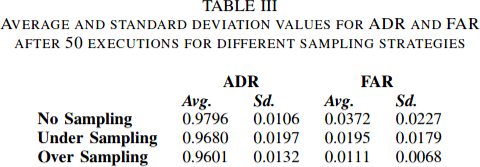
\includegraphics[width=0.7\linewidth,keepaspectratio]{Images/sampling.png}
\caption{Attack Detection Ratio and False Alarm Rate on test data when random samples are removed from the dataset (under sampling) and when random samples are duplicated in the dataset (over sampling) to balance the number of samples in each class. Undersampling is used due to increasing training speed.}
\end{figure}
\end{frame}


%%%%%%%%%%%%%%%%%%%%%%%%%%%%%%%%%%%%%%%%%%%%%%%%%%%%%%%%%%%%%%%%%%%%%%
\begin{frame}[fragile]{Novel Method: State Space Design}
\begin{minipage}[0.2\textheight]{\textwidth}
\begin{columns}[T]
\begin{column}{0.5\textwidth}
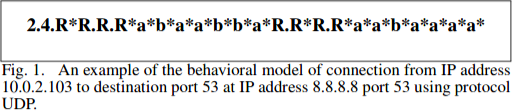
\includegraphics[width=6cm]{Images/example.png}
\\
\vspace{1cm}
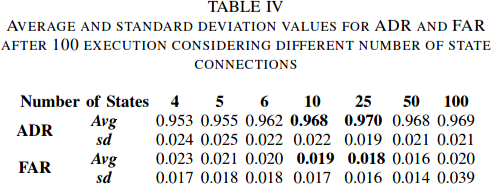
\includegraphics[width=6cm]{Images/conn_len.png}
\end{column}
\begin{column}{0.5\textwidth}
\vspace{.5cm}
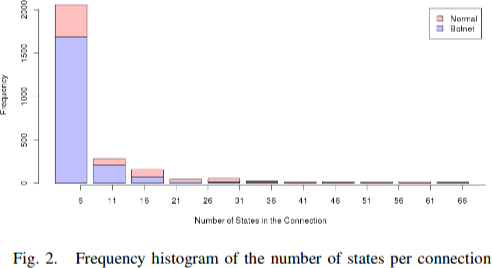
\includegraphics[width=6cm]{Images/hist.png}
\end{column}
\end{columns}
\end{minipage}
\end{frame}



%%%%%%%%%%%%%%%%%%%%%%%%%%%%%%%%%%%%%%%%%%%%%%%%%%%%%%%%%%%%%%%%%%%%%%
\begin{frame}[fragile]{Results}
\begin{figure}
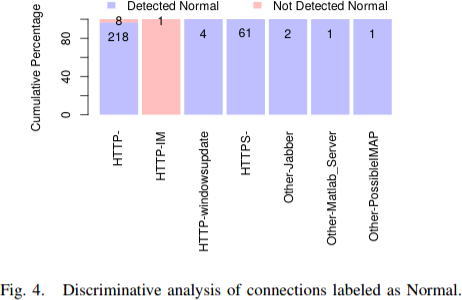
\includegraphics[width=.8\linewidth,keepaspectratio]{Images/normal.png}
\end{figure}
\end{frame}

%%%%%%%%%%%%%%%%%%%%%%%%%%%%%%%%%%%%%%%%%%%%%%%%%%%%%%%%%%%%%%%%%%%%%%
\begin{frame}[fragile]{Results}
\begin{figure}
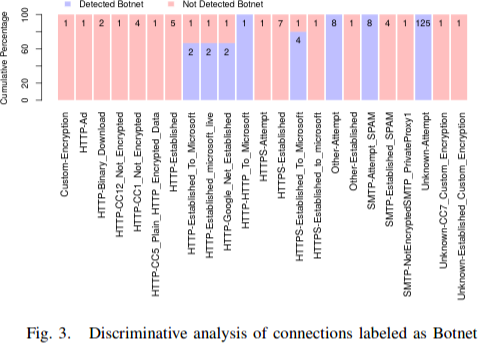
\includegraphics[width=.9\linewidth,keepaspectratio]{Images/botnet_results.png}
\end{figure}
\end{frame}


%%%%%%%%%%%%%%%%%%%%%%%%%%%%%%%%%%%%%%%%%%%%%%%%%%%%%%%%%%%%%%%%%%%%%%
\begin{frame}[fragile]{Conclusion}
\begin{minipage}[0.2\textheight]{\textwidth}
\begin{columns}[T]
\begin{column}{0.5\textwidth}
\begin{itemize}
\item Most all port 80 HTTP- service connections where normal
\item Most all ports with no listed service connections were botnet
\item Data size, periodicity, and duration of TCP connections were not correlated to labels
\item How good was the data set? Can other botnet datasets be classified just off of TCP source port? Seems too simple...
\end{itemize}
\end{column}
\begin{column}{0.5\textwidth}

\includegraphics[width=5cm]{Images/conclusion.png}
\end{column}
\end{columns}
\end{minipage}
\end{frame}


\end{document}